\documentclass{article}

\usepackage{amsmath,amsfonts,amsthm,amssymb}
\usepackage{fancyhdr}
\usepackage{float}
\usepackage{lastpage}
\usepackage{graphicx}
\usepackage{supertabular}
\usepackage{multirow}
\usepackage{ifthen}
\usepackage{enumerate}
\usepackage{subcaption}
\usepackage[hidelinks]{hyperref}
\usepackage{soul}
\usepackage[mediumspace,mediumqspace,squaren]{SIunits}

% In case you need to adjust margins:
\topmargin=-0.5in
\evensidemargin=0in
\oddsidemargin=0in
\textwidth=6.5in
\textheight=9.0in
\headsep=0.25in

% Homework Specific Information
\newcommand{\hmwkTitle}{Project Report 4}
\newcommand{\hmwkDueDate}{May 5th, 2014}
\newcommand{\hmwkClass}{42-731}
\newcommand{\hmwkAuthor}{Alex Sun Yoo, Michael Nye, Ozan Iskilibli}
\newcommand{\hmwkEmail}{ayoo, mnye, oiskilib}
\newcommand{\hmwkCollaborators}{}
\newcommand{\bigspace}{\vspace{.25in}}

% Tools for formatting questions
\newcommand{\question}[1] {\vspace{.25in} \hrule\vspace{0.5em}
\noindent{\bf #1} \vspace{0.5em}
\hrule \vspace{.10in}}
\renewcommand{\part}[1] {\vspace{.10in} {\bf (#1)}}

% Setup the header and footer
\pagestyle{fancyplain}
\lhead{\fancyplain{}{\hmwkAuthor \\ \hmwkEmail}}
\chead{\fancyplain{}{\textbf{\hmwkTitle}}}
\rhead{\fancyplain{}{\hmwkClass \\ Due:\ \hmwkDueDate}}
\lfoot{}
\cfoot{}
\rfoot{Page\ \thepage\ of\ \pageref{LastPage}}
\renewcommand\headrulewidth{0.4pt}
\renewcommand\footrulewidth{0.4pt}

% Format paragraphs to have spacing instead of indents
\setlength{\parindent}{0pt}
\setlength{\parskip}{5pt plus 1pt}

% This is used to trace down (pin point) problems
% in latexing a document:
%\tracingall

\renewcommand{\arraystretch}{1.5}

%%%%%%%%%%%%%%%%%%%%%%%%%%%%%%%%%%%%%%%%%%%%%%%%%%%%%%%%%%%%%

\begin{document}

\thispagestyle{plain}
\begin{center}
{\Large \hmwkClass\ \hmwkTitle} \\
\hmwkAuthor \\
\hmwkEmail \\
\ifthenelse{\equal{\hmwkCollaborators}{}}{}{Collaborators: \hmwkCollaborators\\}
Due: \hmwkDueDate\\
\end{center}
%%%%%%%%%%%%%%%%%%%%%%%%%%%%%%%%%%%%%%%%%%%%%%%%%%%%%%%%%%%%%

\section*{Part 1: Image segmentation using MAT-ITK}

\subsection*{B.1 MAT-ITK and image data}

Our images and their corresponding segmentations are stored in a vector of structs, allowing us to keep all information bundled together.

The MAT\_ITK library is included in our code as a MEX file. We elected to write wrapper functions to convert between our data structs and the format required by the library. This simplifies repeatedly calling the library, as the data format for the library is strange and poorly documented.

It was difficult to find documentation on what function parameters actually were. Fortunately, I was able to find external documentation on how to use some functions\cite{designest}.


\subsection*{B.2.1 Segmentation of static images}

For this assignment, our two assigned algorithms were Connected Threshold Segmentation (CST), and Laplacian Level Set Segmentation (LLSS).

\subsubsection*{Connected Threshold Segmentation}
To perform CST, we must pass in two parameters. The first is a pair of thresholds corresponding to the minimum and maximum values in our segments. The second is a set of seed coordinates, one for each blob we want to segment. For our two test images, these were both derived by manually inspecting the image. See Figures \ref{fig:b21_image1}\&\ref{fig:b21_image2} for results.

\subsubsection*{Laplacian Level Set Segmentation}
To perform LLSS, several parameters were required. The last three had suggested values in the documentation, and we found that the suggested values produced quite good segmentation results. Second, we had to pass in a starting segmentation and a parameter that informs the algorithm what is a segment in the starting segmentation.

LLSS requires an initial segmentation as a seed that it then uses to refine to a better boundary. To seed the algorithm, we used a naive thresholding segment on the image, derived manually by inspecting the image. Finally, the algorithm required a propagation scaling constant. This was manually tuned, and found to produce optimal results between 0 and 1.

\subsection*{Results Comparison}
Both algorithms perform quite well for their simplicity. In both the calibration slide and the cell images, they correctly identify all of the expected foreground features, while rejecting most of the background. LLSS creates a more clean segmentation boundary, and does a better job of rejecting noise around each object; this is most prominent in the cell images in Figure \ref{fig:b21_image2}. However, the cost of this clean segmentation boundary in most cases is that a few internal locations become speckled, rather than a solid region. In contrast, the CST manages to segment the full feature.

The biggest difference is in the work that must go into seeding the image. CST requires manually pinpointing starting seeds inside every object, and determining a threshold for those objects. Meanwhile, LLSS requires only a starting segmentation that somewhat resembles the targeted image; therefore, it can be seeded from a single threshold that need not be precise.

Overall, LLSS produces more desirable results, and has a much easier burden of work placed on the user before it takes place, and so is clearly the stronger algorithm.

\begin{figure}
\centering
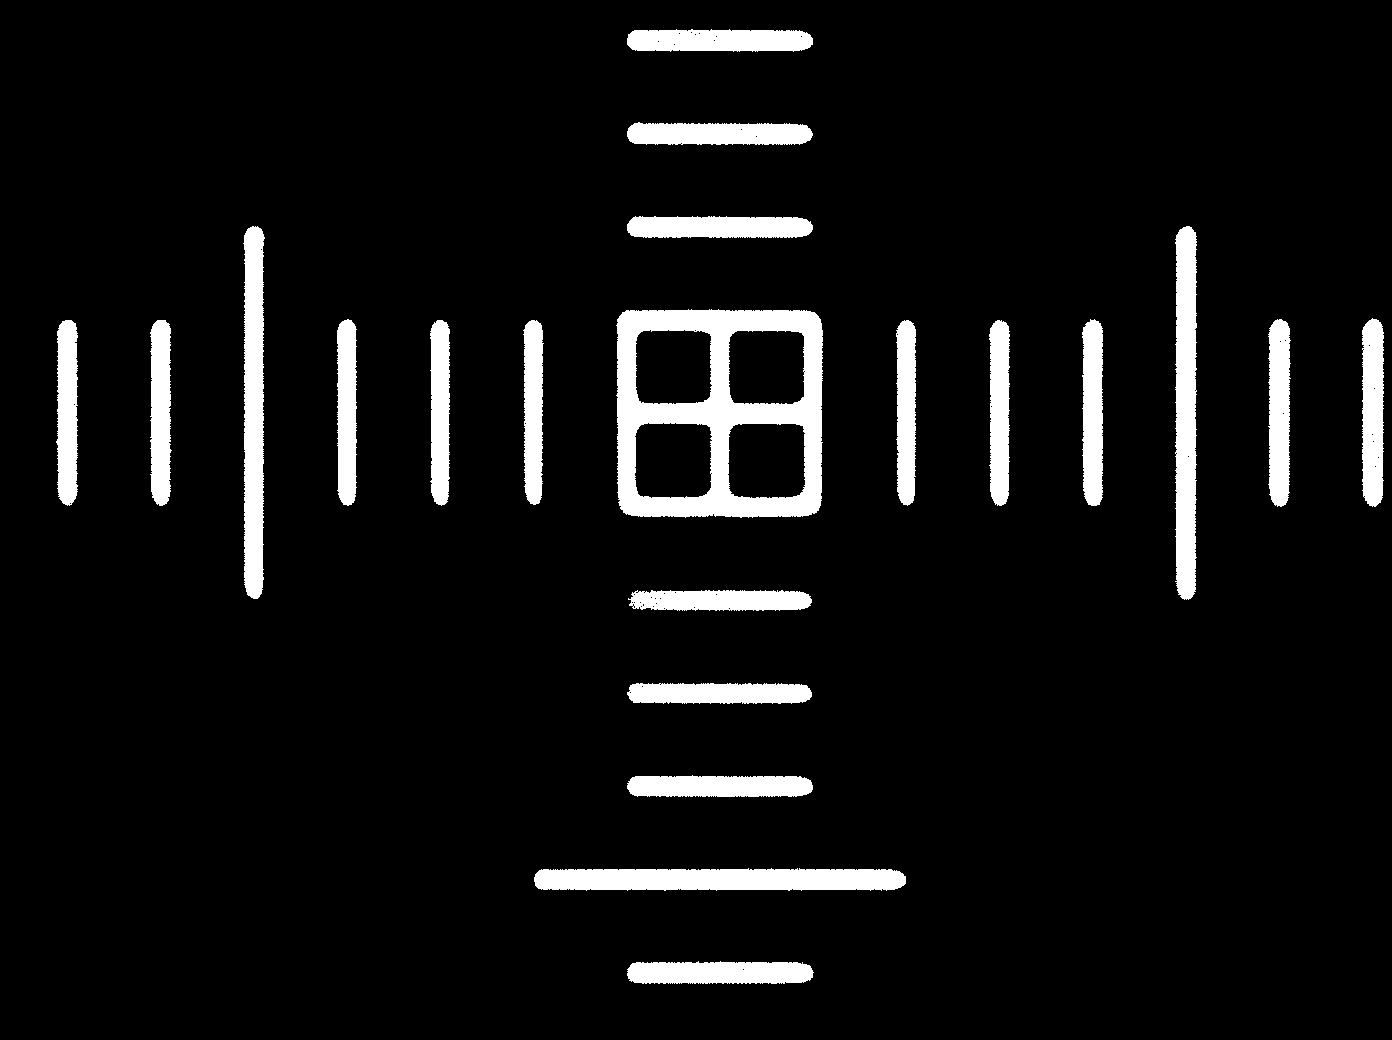
\includegraphics[width=0.4\textwidth]{figures/60x_02_sct.png}
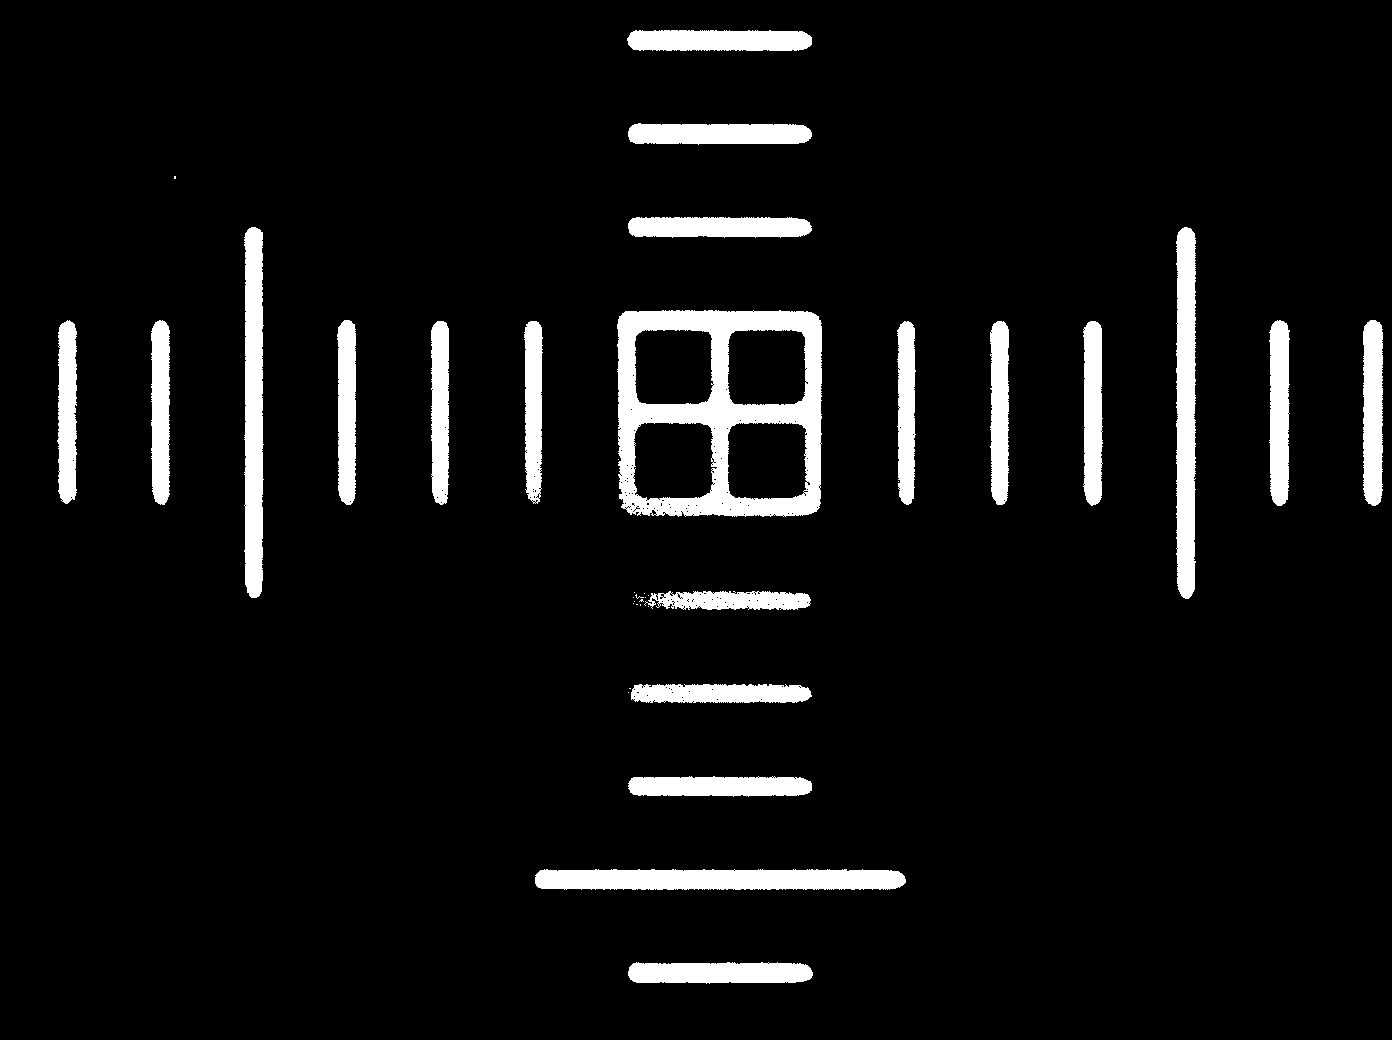
\includegraphics[width=0.4\textwidth]{figures/60x_02_slls.png}
\caption{60x\_02 segmented using CST (left) and LLSS (right)}
\label{fig:b21_image1}
\end{figure}

\begin{figure}
\centering
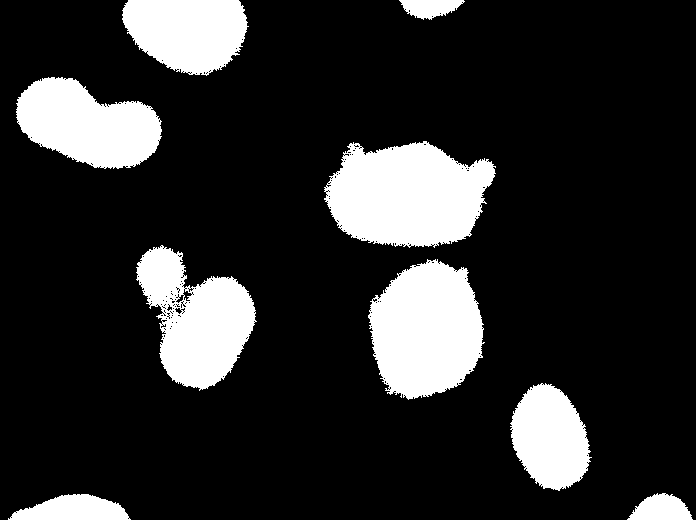
\includegraphics[width=0.4\textwidth]{figures/Blue0001_sct.png}
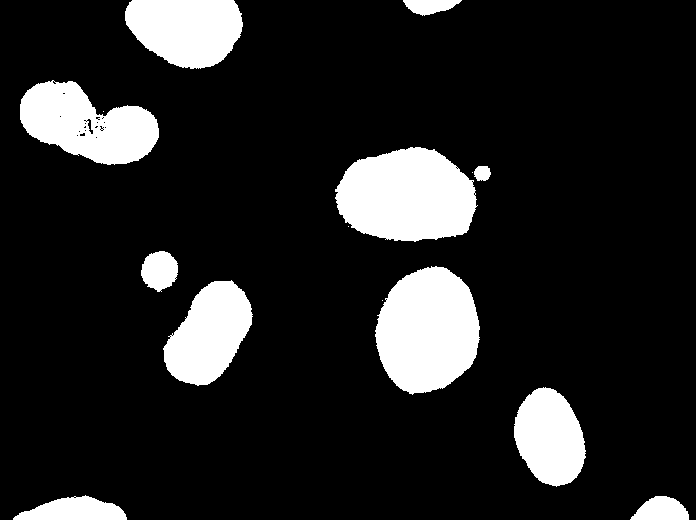
\includegraphics[width=0.4\textwidth]{figures/Blue0001_slls.png}
\caption{Blue0001 segmented using CST (left) and LLSS (right)}
\label{fig:b21_image2}
\end{figure}


\subsection*{B.2.2 Segmentation of images series}

The image series was segmented using the same functions as the in B.2.1. Thresholds were again manually determined by inspecting representative images in the series. The CST was instead seeded using local maxima in the image. See Figure \ref{fig:b21_imageseries} for results.

\begin{figure}
\centering
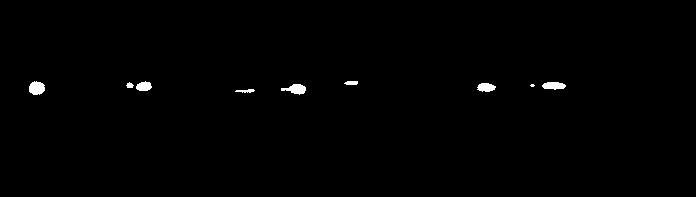
\includegraphics[width=0.8\textwidth]{figures/MitoGFP_LgtGal4_a01r01s02001_sct.png}
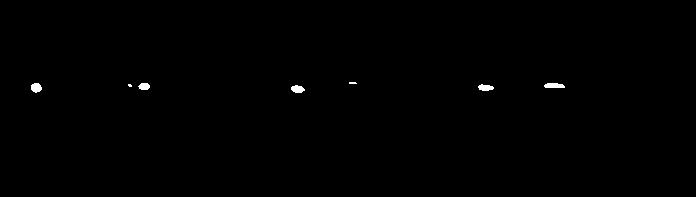
\includegraphics[width=0.8\textwidth]{figures/MitoGFP_LgtGal4_a01r01s02001_slls.png}
\caption{First frame of the image series segmented using CST (top) and LLSS (bottom)}
\label{fig:b21_imageseries}
\end{figure}


\subsection*{B.2.3 Theoretical background}

\subsubsection*{Connected Threshold Segmentation}
Connected Threshold Segmentation is a very simple algorithm. It begins with one or more starting coordinates, called the {\bf seeds}. For each seed location, we search the neighborhood around the point. The most common neighborhood is simply the eight adjacent pixels. For each grayscale pixel, we compare against two thresholds, $T_L$ and $T_H$. If the pixel intensity $p_i$ is in the range $T_L \leq p_i \leq T_H$, then this pixel is added to the segmentation. Finally, for each pixel found this way, iteratively continue expanding the segmentation. The algorithm terminates when no new pixels are found in the next iteration step.\cite{svi}

This algorithm is incredibly simple, and thus easy both to implement and tune the parameters for. In the case of our clean test images, it actually produces quite clean results with minimal effort. However, it requires that the user feeds the algorithm with knowledge for each image that describes the segments, meaning it is hard to fully automate.

\subsubsection*{Laplacian Level Set Segmentation}
Level set segmentation derives form a mathematical property called the level set. A level set is simply the set of all points for a function $f$ where $f(x) = c$, where $c$ is some constant. Level set algorithms define the ``interface'' as the dividing line between a segment and everything else, and seeks to define a function $\varphi(\mathbf{x},t)$ such that $\varphi$ is strictly positive (or negative) when inside a segment, strictly negative (or positive) outside a segment, and strictly $0$ on the dividing line. Thus, the segmentation can be found by finding the level set $\Gamma(t)$ that causes $\varphi$ to {\emph vanish} (that is, to go to zero).

To perform optimization, a velocity field is defined $\mathbf{v}(\mathbf{x},t)$. Thus, we evolve the equation\cite{osher}:

\[\frac{\delta\varphi}{\delta t} + \mathbf{v} \nabla\varphi = 0 \]

Using Lagrangian methods, this is done by evolving particle positions to track the interface. Starting at an initial position $\mathbf{x_0}$, with an initial volume of segmentation $v_0$, on the initial boundary, we update our state on the next $p$th step as follows\cite{hieber}:

\[\frac{D\varphi_p}{Dt} = 0 \]
\[\frac{Dv}{Dt} = \left< \nabla\mathbf{v}\right>_p v_p \]
\[\frac{D\mathbf{x}_p}{Dt} = \mathbf{v}_p \]

By iterating this for each point on our segmentation boundary, we will eventually converge on our final boundary. The advantage of using particle based adjustment of these boundaries is that they allow for fast and relatively accurate approximations of our actual surface we are traversing. Their primary disadvantage is that sometimes, points can get caught in ``snags'' along their path that causes them to converge to suboptimal locations. This is usually a result of accumulated errors in the approximation of our distance function, and it can be fixed reinitializing our sets by recomputing initial values at our current position and continuing\cite{hieber}.

LLSS as an algorithm is very good at adjusting existing edges that are near actual segmentations. However, because the gradients tend to be small far from edges, it is not as good at guessing initial boundaries and crossing wide spaces\cite{osher}. Thus, given very rough or noisy segmentations by other methods, LLSS makes an excellent second pass to produce clean segmentations.












\clearpage
\section*{Part 2: Image segmentation using graph-cut and active contour}

\subsection*{C.1.1 Graph cut based image segmentation}



Examples of N-Cut Image Segmentation on the two static sample images are shown in figures \ref{fig:gc1_1} and \ref{fig:gc1_2}. The code used to run this algorithm on these images are from reference \cite{ncut_code}.

\begin{figure}
\centering
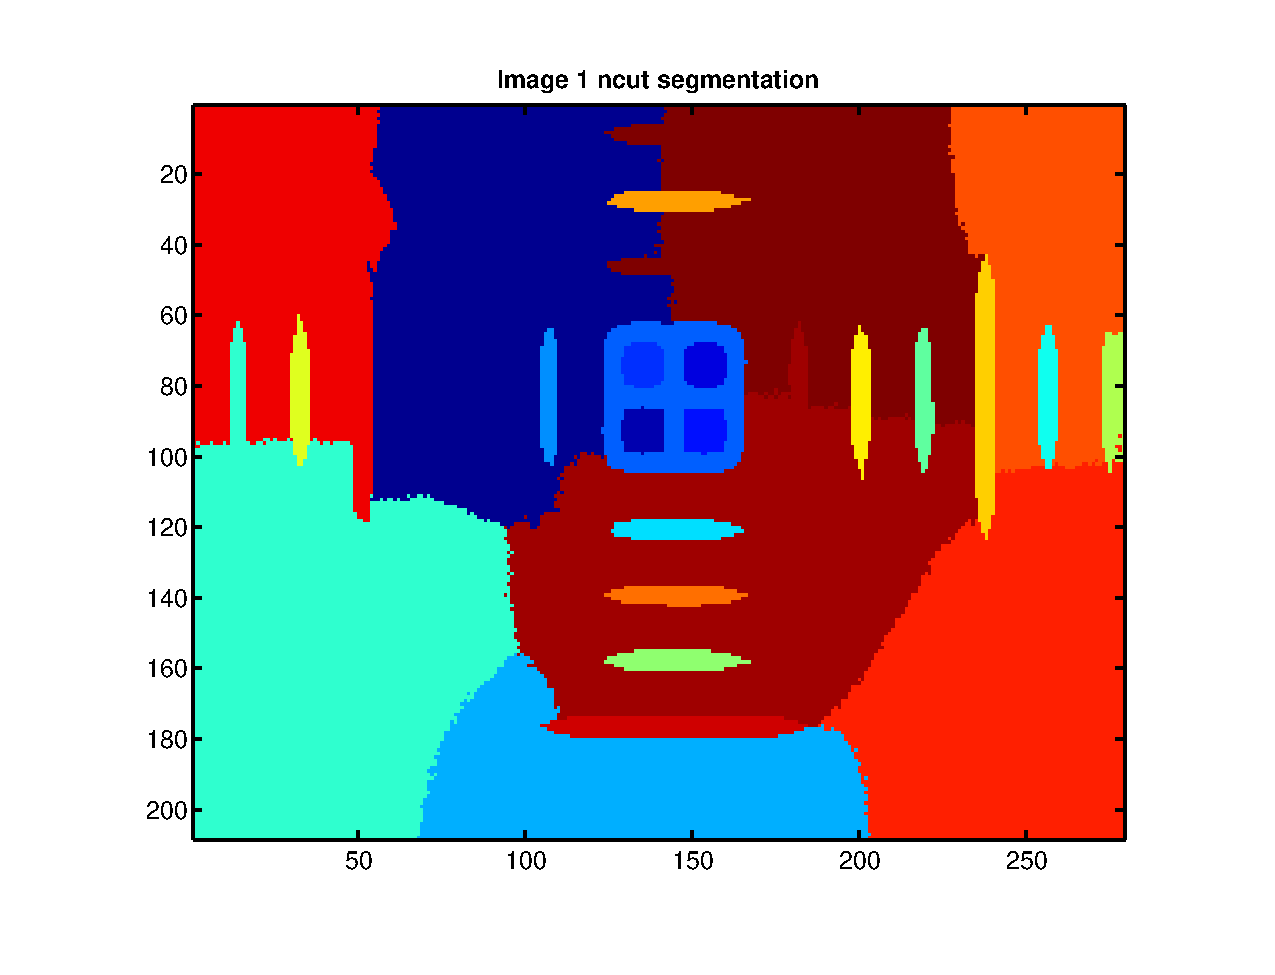
\includegraphics[width=0.5\textwidth]{figures/60x_02_gc1.pdf}
\caption{60x\_02 segmentation using N-Cut Image Segmetation}
\label{fig:gc1_1}
\end{figure}

\begin{figure}
\centering
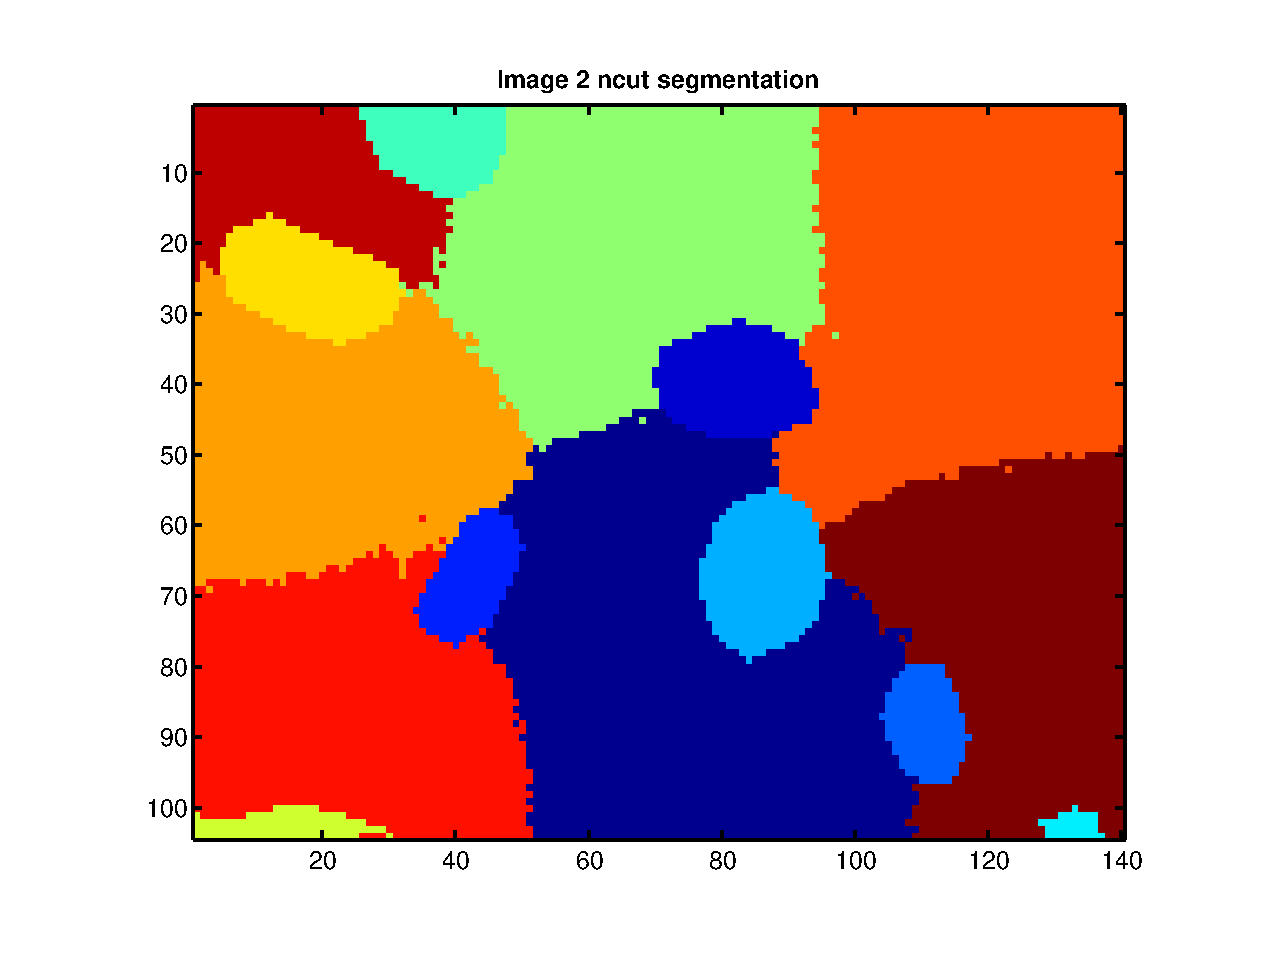
\includegraphics[width=0.5\textwidth]{figures/Blue0001_gc1.pdf}
\caption{Blue0001 segmentation using N-Cut Image Segmetation}
\label{fig:gc1_2}
\end{figure}



 The code used in this project (also provided by \cite{jun}) follows the convexification of the CV algorithm, which partitions "an image into $K$ parts by using $\text{log}_2 K$ level set functions" \cite{jun}. 

Results for the initial two images are in figures \ref{fig:gc2_1} and \ref{fig:gc2_2}.

\pagebreak
\begin{figure}
\centering
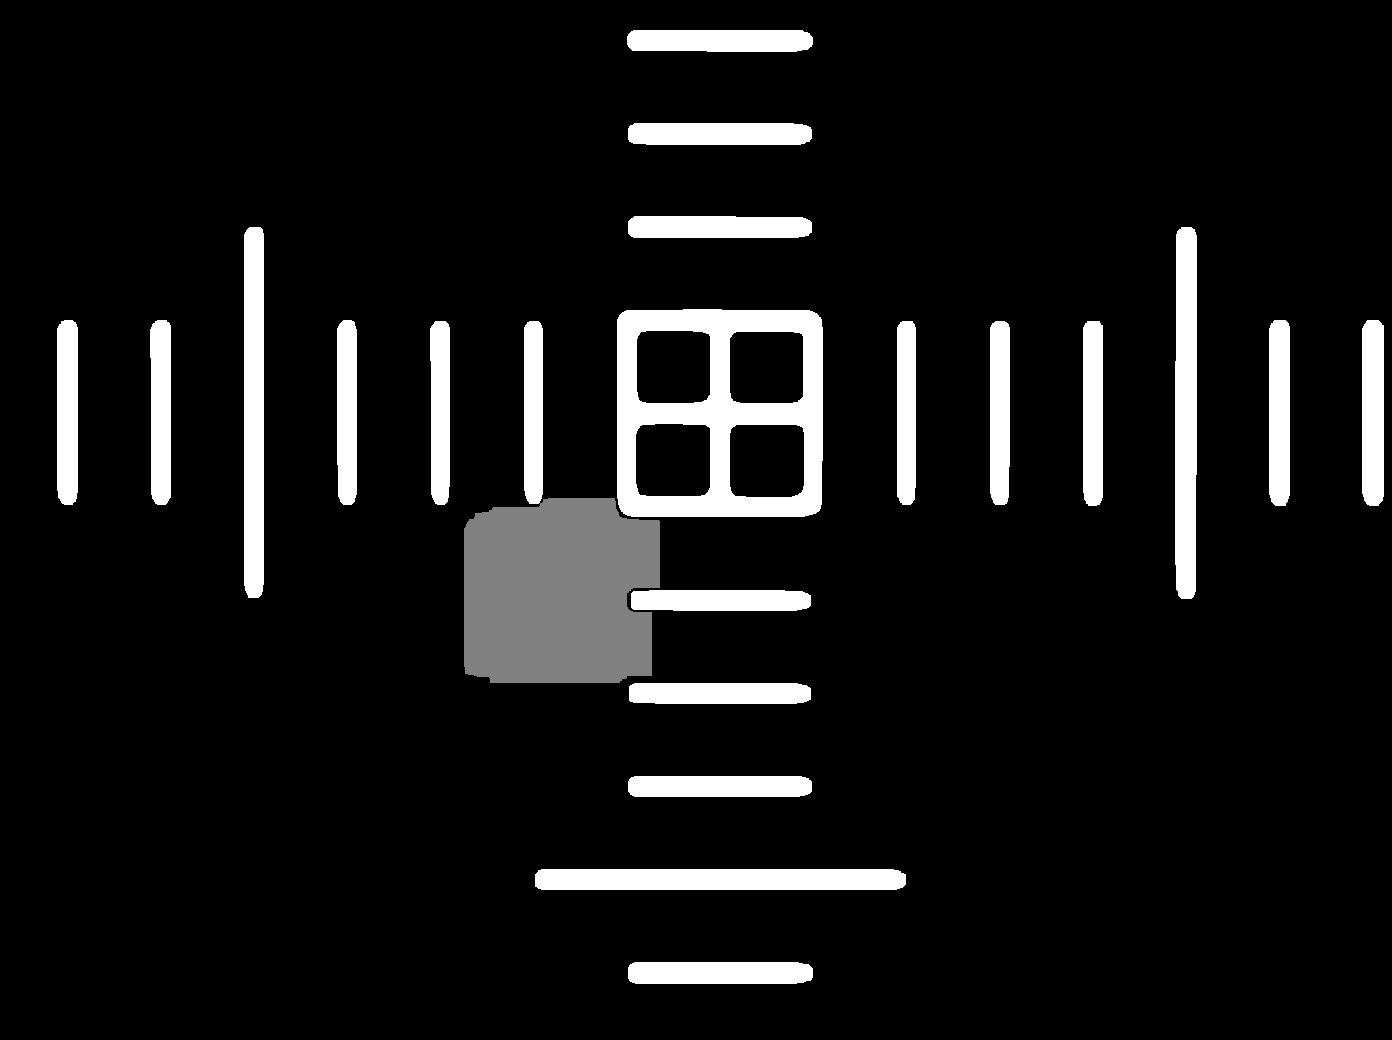
\includegraphics[width=0.5\textwidth]{figures/60x_02_gc2.png}
\caption{60x\_02 segmentation using Convexified CV Image Segmetation}
\label{fig:gc2_1}
\end{figure}

\begin{figure}
\centering
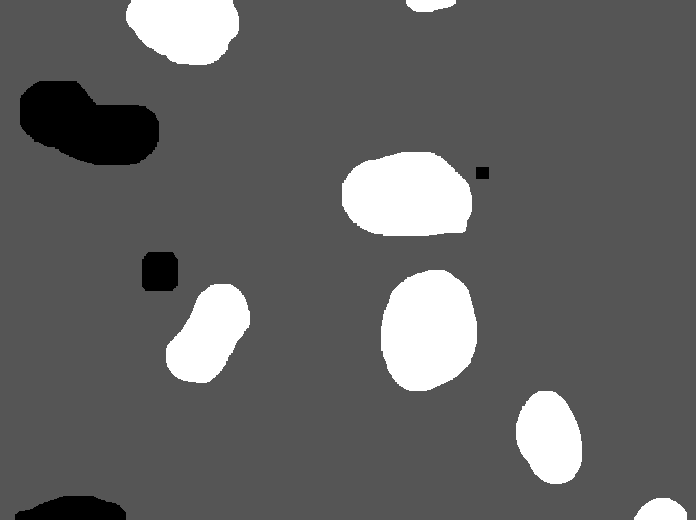
\includegraphics[width=0.5\textwidth]{figures/Blue0001_gc2.png}
\caption{Blue0001 segmentation using Convexified CV Image Segmetation}
\label{fig:gc2_2}
\end{figure}











\pagebreak
\subsection*{C.1.2 Active contour based image segmentation}
Active contours, or \emph{snakes}, are quite useful for finding object boundaries in an image. The initial contours are evolving due to the internal, elastic forces holding the curve together, bending forces controlling stiffness of the curve, and external forces, that are potential forces due to image gradients and pressure forces. Reference \cite{gvf} indicates that there are 2 main challenges in active contour based image segmentation:
\begin{itemize}
\item Initial contours should start in the vicinity of the true region boundaries
\item It is generally hard to penetrate into concave regions.
\end{itemize}
In this project, Gradient Vector Flow Segmentation (GVF) \cite{gvf} and Distance Regularized Level Set Evolution (DRLSE) Segmentation \cite{drlse} are examined and applied to the current sample images, in order to exemplify the functionality and challenges in active contour based image segmentation. In the following, the results and the implementation of each algorithm will be discussed, however, the technical background will be given in section C.1.3. 


\subsubsection*{Gradient Vector Flow Segmentation}
The GVF segmentation has several inputs from the user. First, it needs the initial snake entered by the user. The snake deformation starts from this initial curve. Second, it needs some weighting parameters to evaluate the deformed curve. These parameters are, $\mu$, a parameter that weights the GVF strength, $\alpha$, that weighs the tension of the curve and $\beta$ that controls the rigidity of the snake. These parameters are chosen as $0.2$, $0.05$ and $0.1$ respectively, according to \cite{gvf} and optimized for practical reasons. Resulting figures are available in figures \ref{fig:gvf1p1}-\ref{fig:gvf3}.

\begin{figure}
\centering
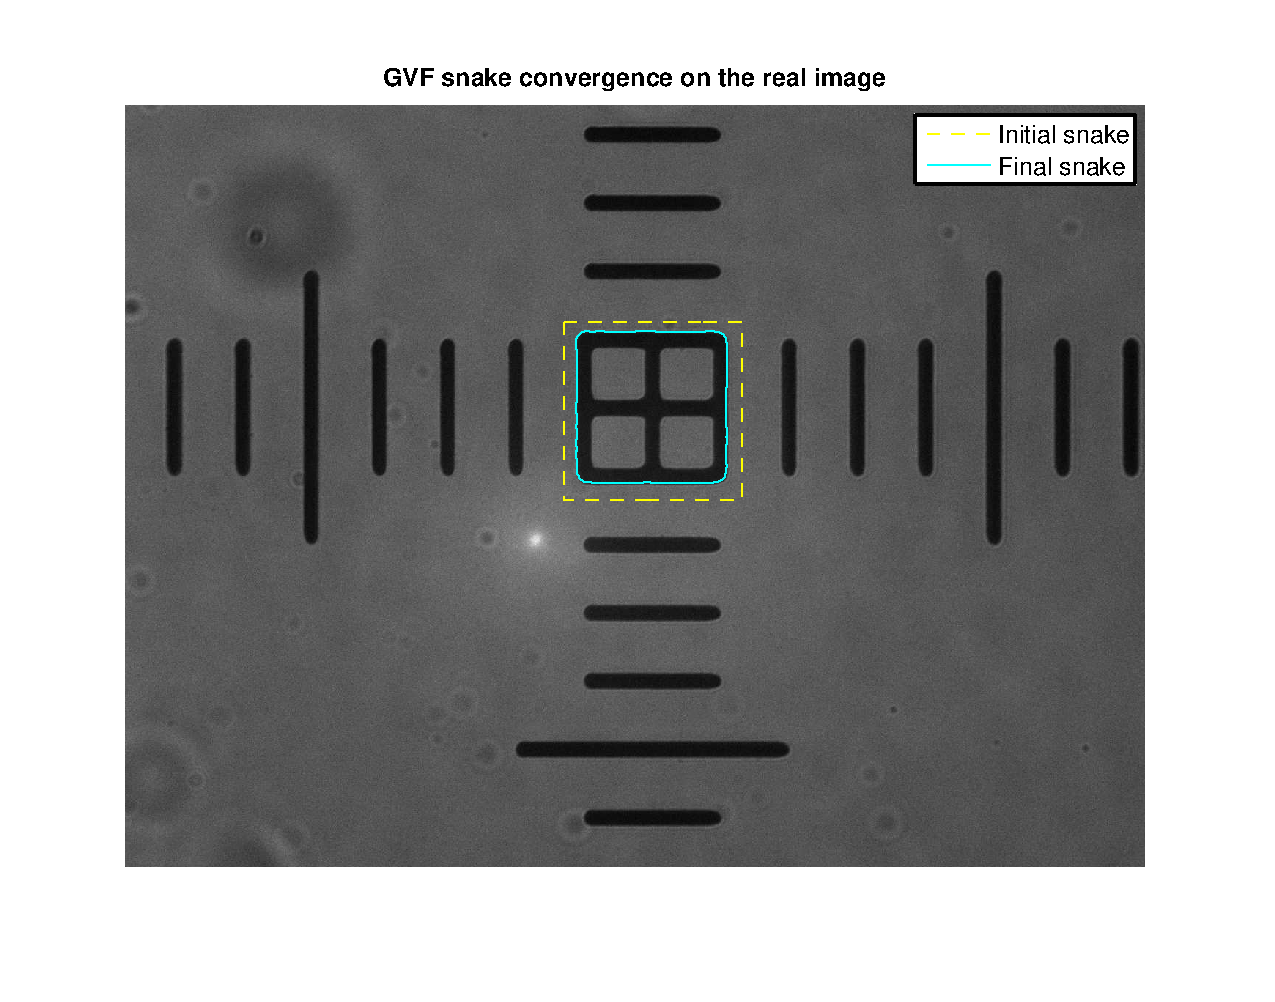
\includegraphics[width=0.85\textwidth]{figures/gvf_1p1.pdf}
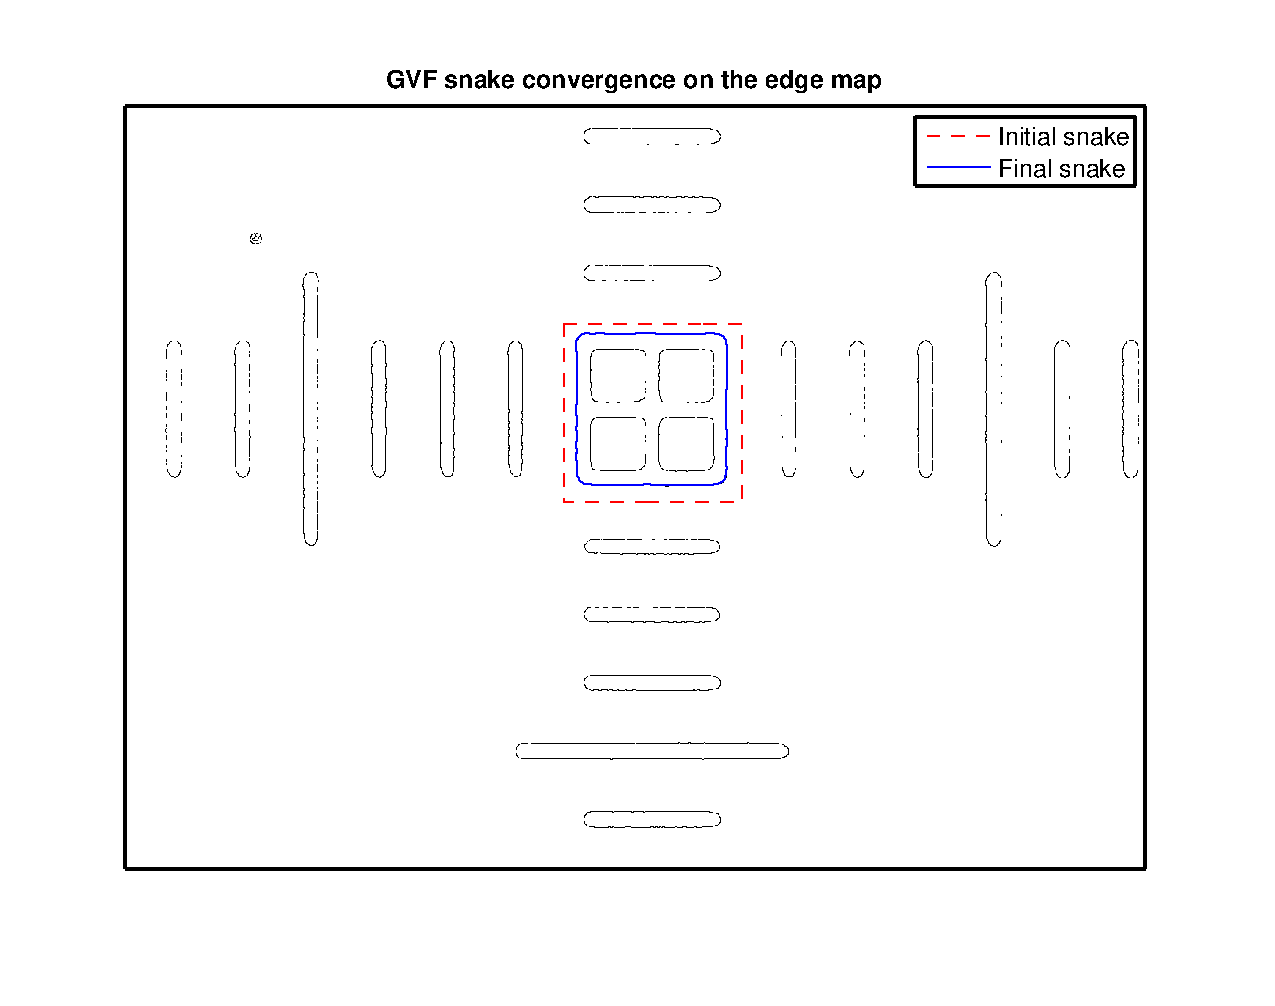
\includegraphics[width=0.85\textwidth]{figures/gvf_1p1_edge.pdf}
\caption{60x\_02 segmented using GVF (top) and projection on the edge map (bottom)}
\label{fig:gvf1p1}
\end{figure}

\begin{figure}
\centering
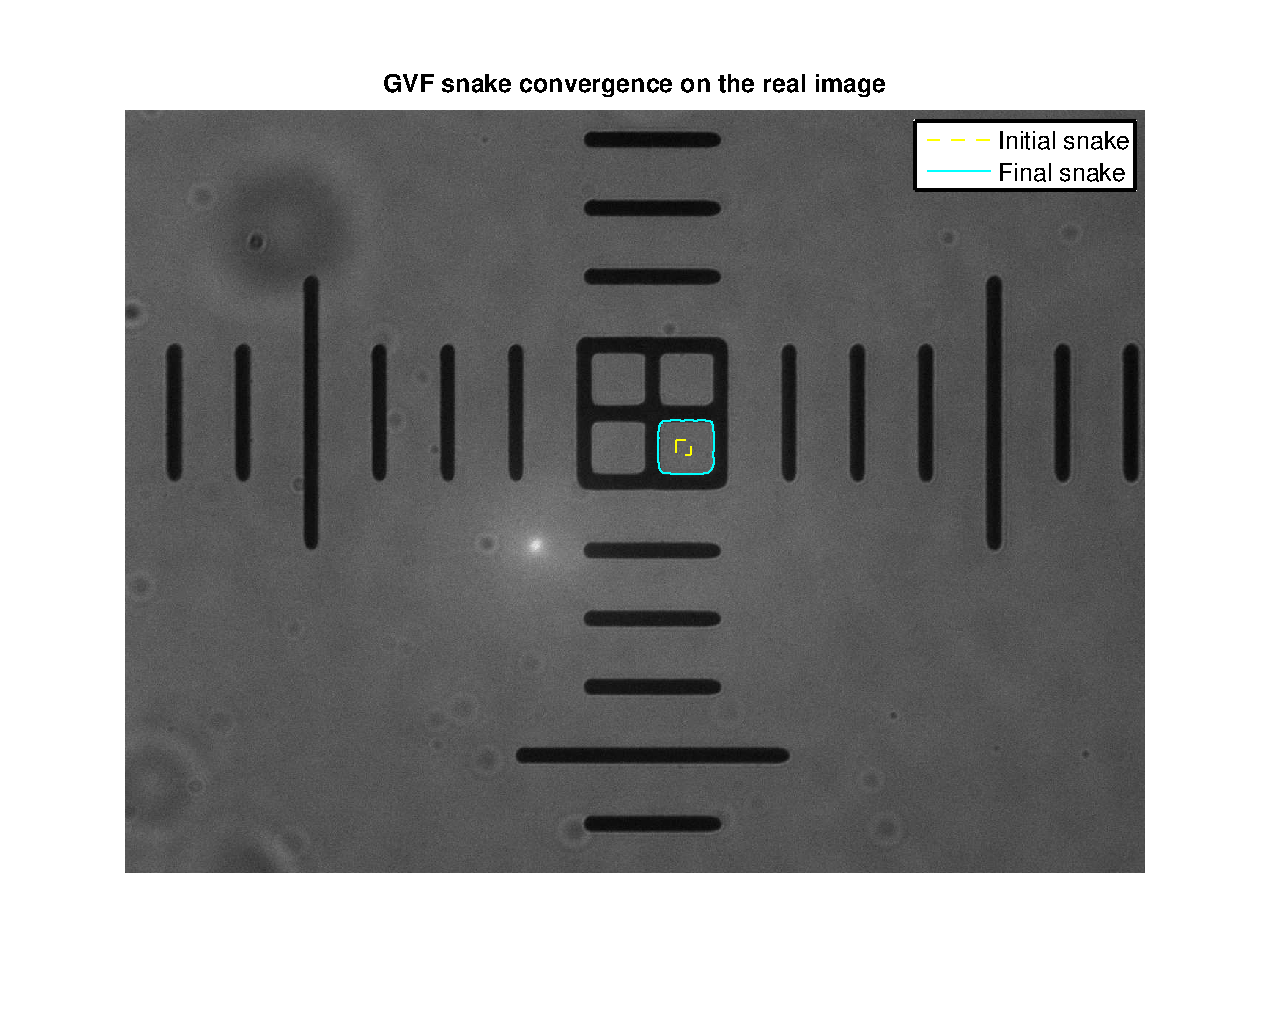
\includegraphics[width=0.85\textwidth]{figures/gvf_1p2.pdf}
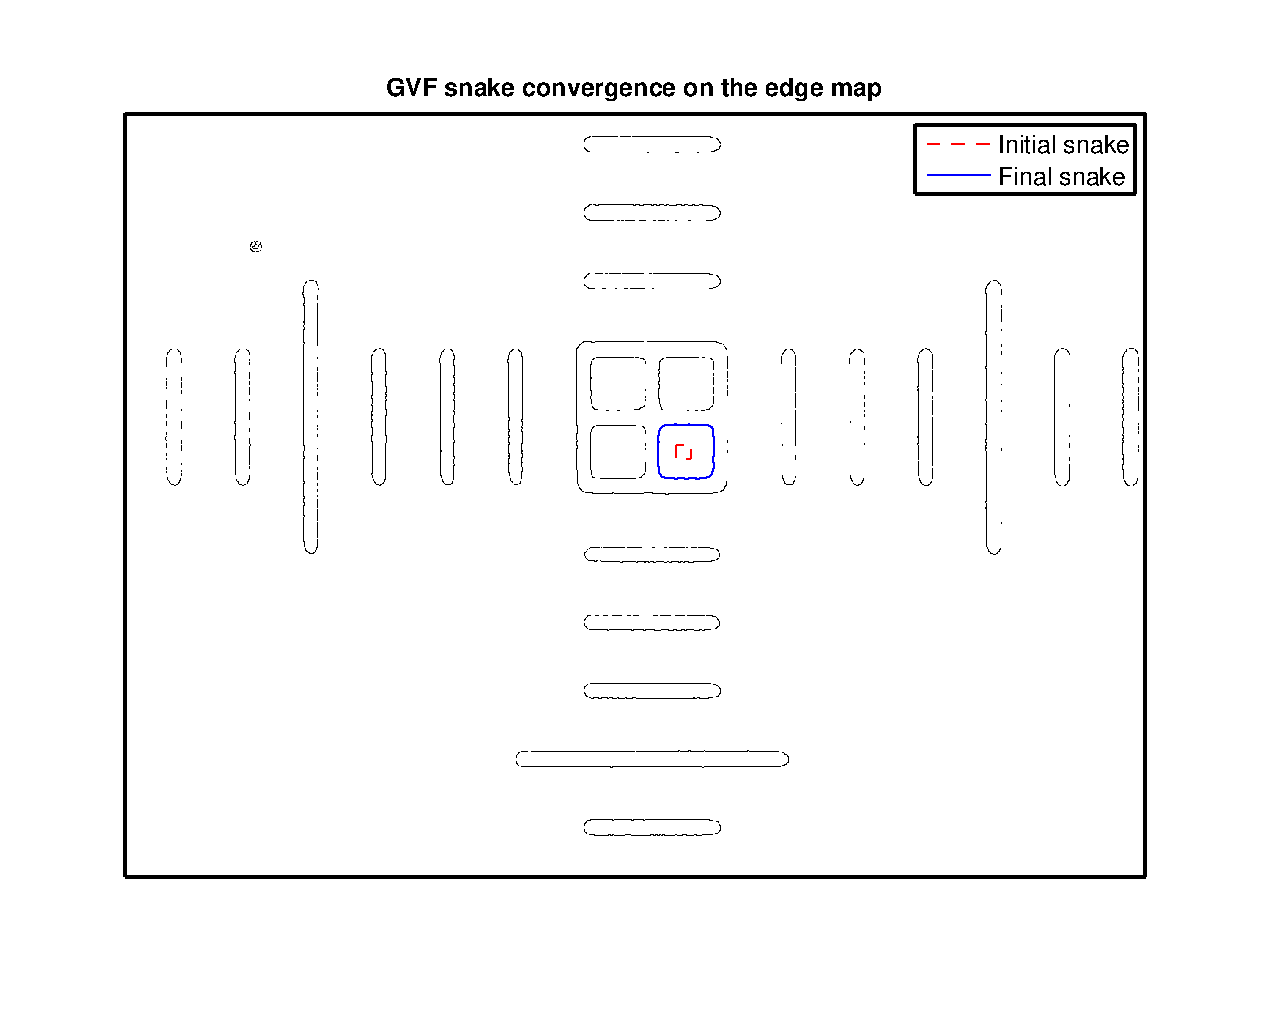
\includegraphics[width=0.85\textwidth]{figures/gvf_1p2_edge.pdf}
\caption{60x\_02 segmented using GVF (top) and projection on the edge map (bottom)}
\label{fig:gvf1p2}
\end{figure}

\begin{figure}
\centering
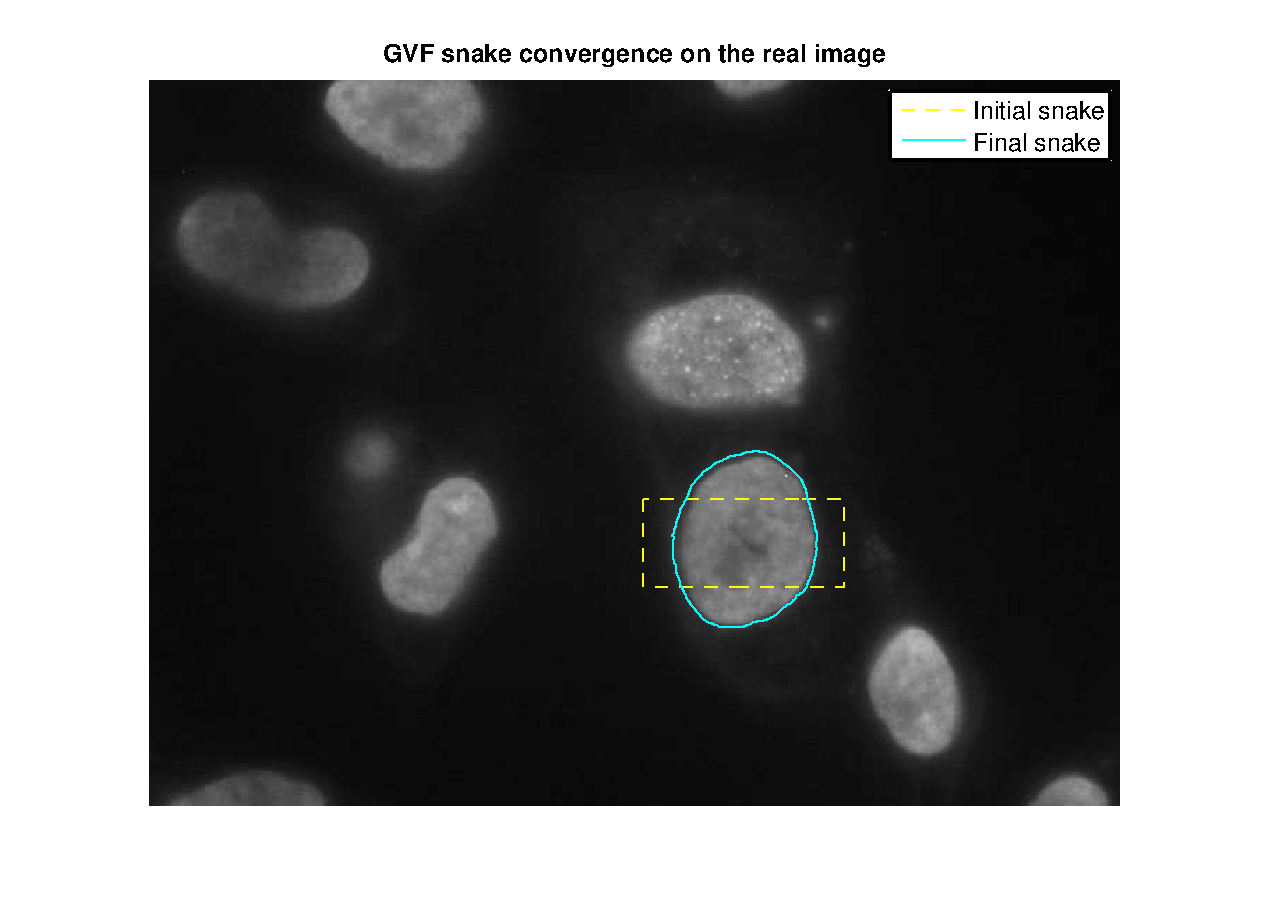
\includegraphics[width=0.85\textwidth]{figures/gvf2.pdf}
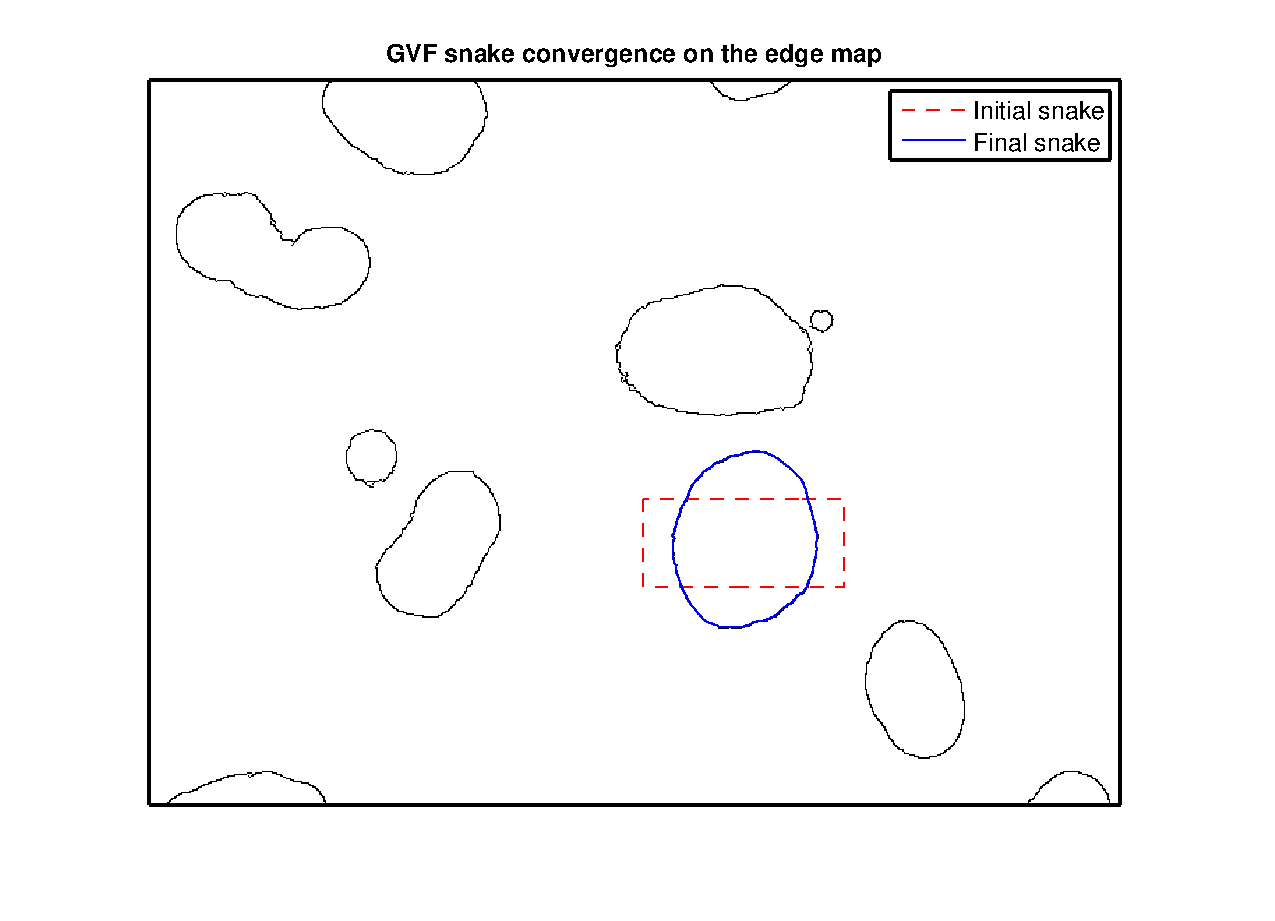
\includegraphics[width=0.85\textwidth]{figures/gvf2_edge.pdf}
\caption{Blue0001 segmented using GVF (top) and projection on the edge map (bottom)}
\label{fig:gvf2}
\end{figure}


\begin{figure}
\centering
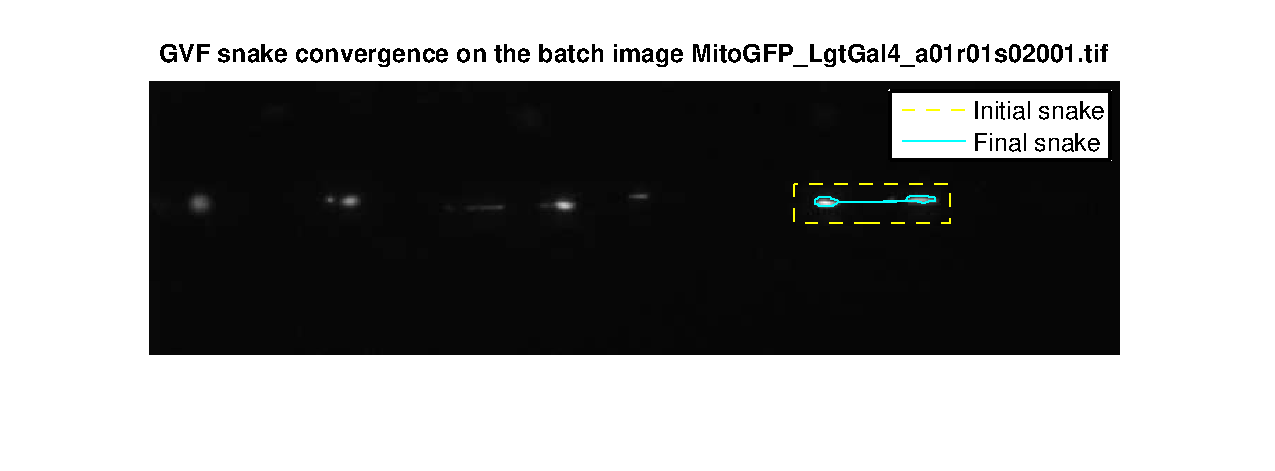
\includegraphics[width=0.85\textwidth]{figures/gvf3.pdf}

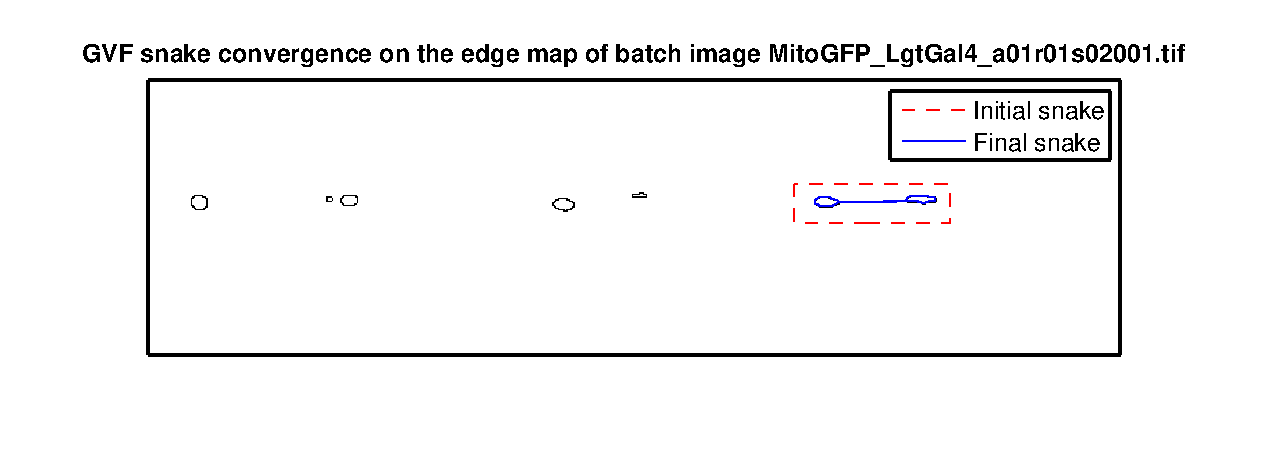
\includegraphics[width=0.85\textwidth]{figures/gvf3_edge.pdf}
\caption{First frame of image series segmented using GVF (top) and projection on the edge map (bottom)}
\label{fig:gvf3}
\end{figure}



\subsubsection*{Distance Regularized Level Set Evolution Segmentation}
The DRLSE segmentation needs to have an initial guess at the segmentation boundary, that is entered by the user, same as the GVF. Because the DRLSE algorithm has some more flexibility in the snake deformation, the algorithm is modified to ask for 2 regions as user's initial guess. The initial contour is the combination of these 2 regions. In that way, the DRLSE's performance could be observed easier in cases such as region delineation. In addition, the function calls of the developed algorithm asks for parameters such as time step for evolution, length and area weights of the cost function and some other parameters, which are all set according to the examples in \cite{gvf} and adjusted for practical reasons when necessary. This necessity arises when the image contains significantly more pixels than other sample images, such that the simulation time is inadequate to converge feature boundaries. In order to effectively run these algorithms, above explained parameters are normalized according to number of pixels in images, for each image. In practice, the evolution is at a similar pace in terms of CPU time but much faster in terms of snake deformation in pixels per evolution step, for larger images. Obviously, this results in loss of weak features in large images, but worked out well in this project. The resulting segmentations are available in figures \ref{fig:drlse1}-\ref{fig:drlse3}. 

\begin{figure}
\centering
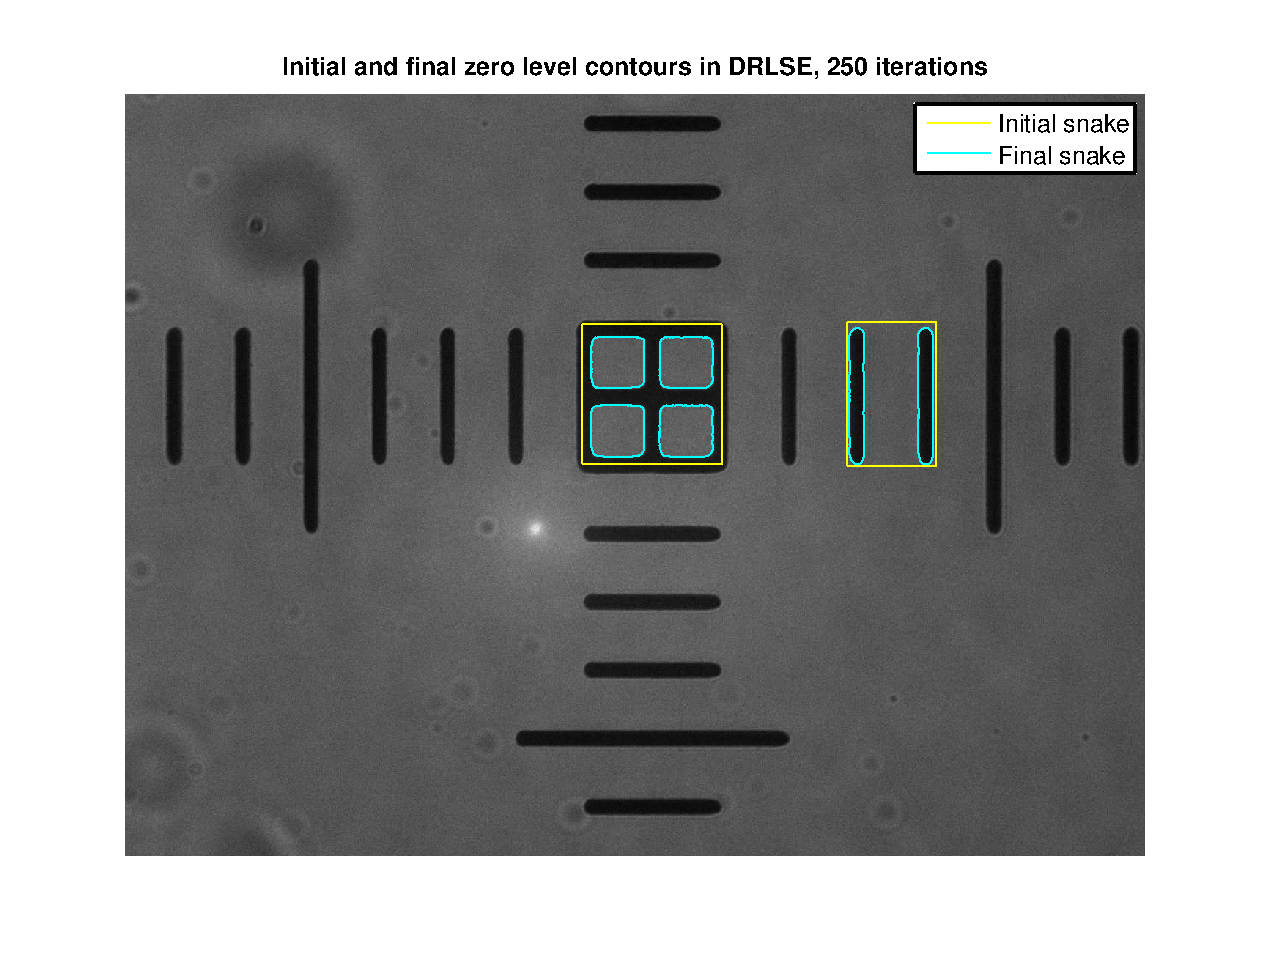
\includegraphics[width=0.85\textwidth]{figures/drlse1.pdf}
\caption{60x\_02 segmented using DRLSE}
\label{fig:drlse1}
\end{figure}

\begin{figure}
\centering
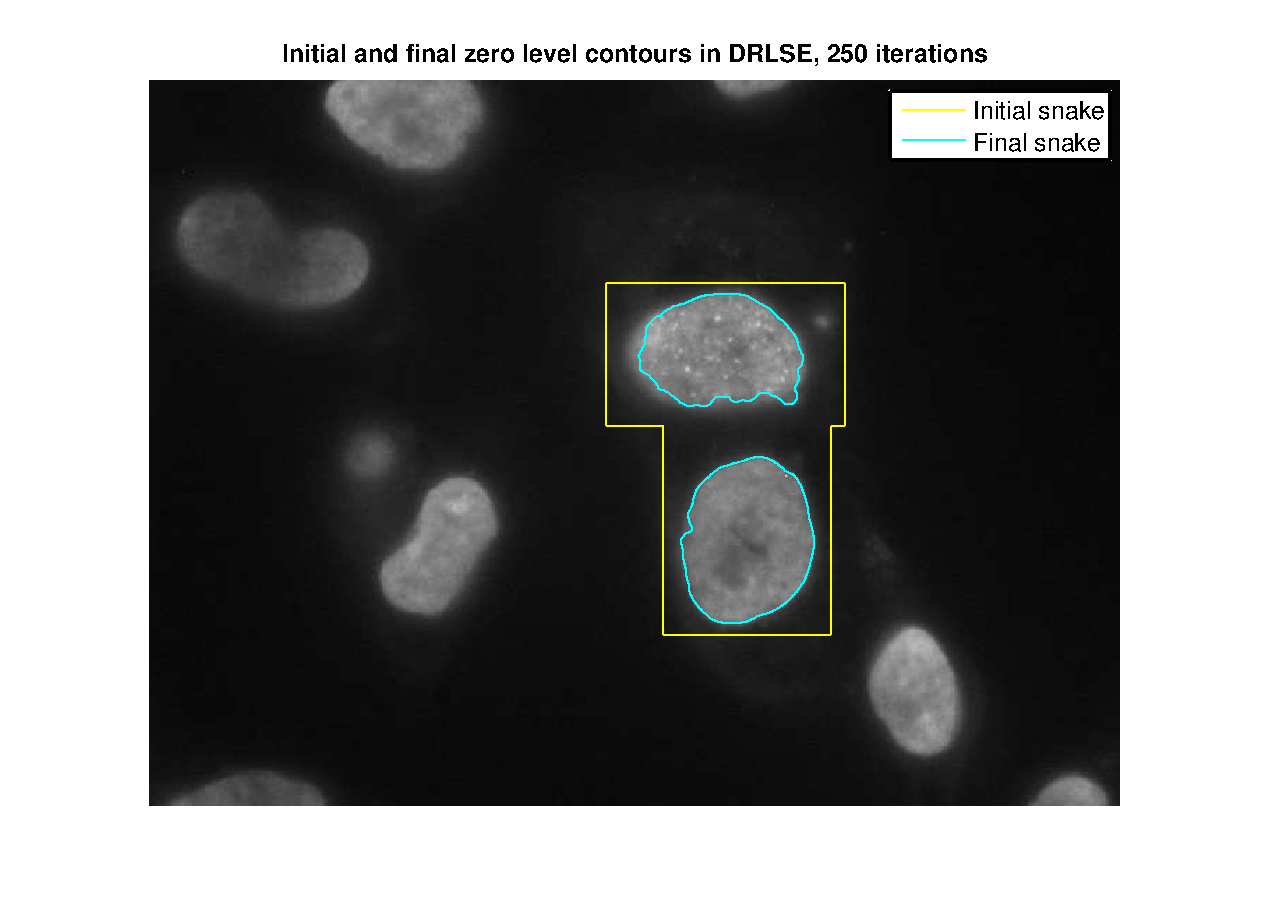
\includegraphics[width=0.85\textwidth]{figures/drlse2.pdf}
\caption{Blue0001 segmented using DRLSE}
\label{fig:drlse2}
\end{figure}


\begin{figure}
\centering
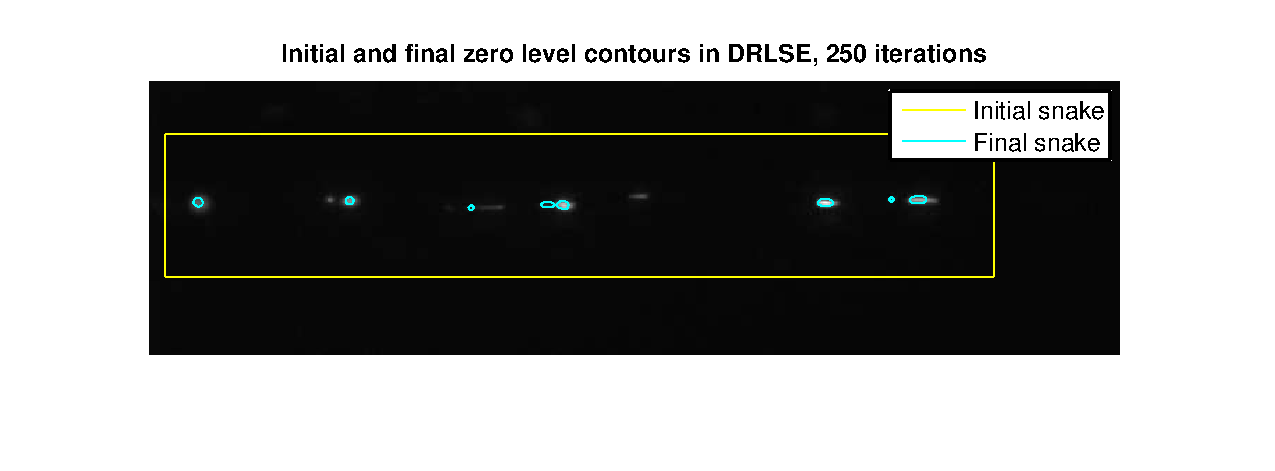
\includegraphics[width=1\textwidth]{figures/drlse3.pdf}
\caption{First frame of image series segmented using DRLSE}
\label{fig:drlse3}
\end{figure}



\subsubsection*{Results Comparison}
Each algorithm performs really well on sample images, although they each have their natural limitations. These algorithms will be compared in 3 aspects: direction of the snake deformation, segmenting multiple regions within an initial guess and reliability.

Firstly, the direction of the snake deformation will be examined. The GVF snake moves towards image gradients, meaning every possible direction. Shrinking and expanding are observable when figures \ref{fig:gvf1p1} \& \ref{fig:gvf1p2} are compared, while figure \ref{fig:gvf3} standalone illustrates shrinking in some directions and expanding other directions. On the other hand, the DRLSE snake has its direction hard-coded and that is inwards,  i.e. shrinking, in our implementation. That is why in all of figures \ref{fig:drlse1}-\ref{fig:drlse3}, the initial guess is always encapsulating objects to be segmented, instead of lying inside the objects.

Secondly, the segmentation of multiple objects that fall within the same initial guess will be compared. If the GVF initial guess contains multiple objects, the algorithm will encapsulate each region and diffuse into the area in between disjoint regions. However, the GVF does not have a property to divide itself into multiple regions, therefore the final snake looks like few segmented regions attached by a string, as seen in figure \ref{fig:gvf3}. On the other hand, the DRLSE naturally divides into multiple regions and detects separate objects easily: in figure \ref{fig:drlse1} it divides into 4 regions on the left and 2 regions on the right,while in figure \ref{fig:drlse3} an exaggerated large initial snake returns 8 detected objects in the image.

Lastly, the GVF shows pretty good convergence to the detected edges. In fact, the GVF is built to stop snake deformation when the detected edges are reached, so if the GVF convergence looks messy, the problem is simply the edge detection. This behavior is observable in bottom plots (edge maps) of figures \ref{fig:gvf1p1}-\ref{fig:gvf3}. On the other hand, the DRLSE works on an energy function that has only a weighted ``edge indicator'' (theory is explained below in part C.1.3). Therefore, DRLSE needs some correction steps, where the energy function disregards the external forces for deformation and tries to find its equilibrium. This balancing step does not show up in theoretical results, but applied for practical reasons. Effectively, the DRLSE outcome could have some leakage into the true object boundaries and that is partly observable in figure \ref{fig:drlse2}, as there are some grayish area left outside the segmented regions.


\subsection*{C.1.3 Theoretical background}



\subsubsection*{Normalized Cuts in Image Segmentation}

The general concept of using graph cuts for image segmentation is to use a weighed graph to represent the entire image, such that each vertex represents one pixel of the image, and each edge's weight is a scalar that is a function of some factor of similarity between the two vertices. If the image is partitioned into two whole segments, then a graph cut for that partionining is defined as the sum of weights between every combination of pairs of vertices between the two regions, as shown in equation \ref{eq:graph_cut}.

\begin{equation}
cut(A,B) = \sum_{u\in A,v\in B} w(u,v)
\label{eq:graph_cut}
\end{equation}
...such that $A$ and $B$ are the set of vertices in their respective regions of the given image, and the function $w(u,v)$ is the weight between vertices $u,v$.

Typically, the ideal partioning into regions $A$ and $B$ is one that minimizes the cut, so the two regions are as distinguishable as possible from each other, implying good segmentation (this is called finding the minimum-cut). There are other methods of taking advantage of graph cuts, or uses a similar idea, however. Two such methods are normalized cuts and non-convex.

Rather than calculating and using equation \ref{eq:graph_cut}, however, Shi and Malik formulated the normalized cut (or N-cut), which "computes the cut cost as a fraction of the total edge connections to all the nodes in the graph" \cite{ncut}. The normalized cut formula for dissociation is given below in equation \ref{eq:norm_cut1}: \cite{ncut}

\begin{equation}
Ncut(A,B) = \frac{cut(A,B)}{assoc(A,V)} + \frac{cut(A,B)}{assoc(B,V)}
\label{eq:norm_cut1}
\end{equation}

where $assoc(A,V) = \sum_{u\in A, t\in V} w(u,t)$, or the "graph cut" between region $A$ and the entire graph itself; the idea behind this is to perform segmentation based off of not only each partition's relationship with each other, but also relationship to the entire image \cite{ncut}. The normalization cut addresses the issue with the minimization cut in equation \ref{eq:graph_cut} where it favors partitioning out sets of isolated vertices.

The normalized cuts algorithm also calculates the total normalized association within the partitions themselves, which is given in equation \ref{eq:norm_cut2}: \cite{ncut}

\begin{equation}
Nassoc(A,B) = \frac{assoc(A,A)}{assoc(A,V)} + \frac{assoc(B,B)}{assoc(B,V)}
\label{eq:norm_cut2}
\end{equation}

The association and dissociation in equations \ref{eq:norm_cut1} and \ref{eq:norm_cut2} are also directly related: \cite{ncut}

\begin{equation}
Ncut(A,B) = 2 - Nassoc(A,B)
\end{equation}

This relationship makes the partitioning criteria more trivial, as maximizing one minimizes the other. For an ideal segmentation with the N-cut algorithm, the dissociation in equation \ref{eq:norm_cut1} should be maximized and the association in equation \ref{eq:norm_cut2} should be minimized.




\subsubsection*{Convex Multiphase Image Segmentation with Graph Cut}

The image segmentation algorithm used by \cite{jun} is another algorithm based off of graph cut that minimizes the global energy via convexifying the non-convex cost functions.

Graphically, a convex function is one where graphically, the line segment between any two points on the function is above the function itself (or just below; one or the other). Simple low-dimensional examples include $f(x)=x^2$, $f(x)=e^x$ and so on. A non-convex function is one where this property does not hold. The mathematical definition is provided in equation \ref{eq:convex} \cite{convex}.

\begin{equation}
\forall x_1,x_2 \in X, \forall t\in [0,1]: f(tx_1 + (1-t)x_2 \leq tf(x_1) + (1-t)f(x_2)
\label{eq:convex}
\end{equation}

where $x_1,x_2$ are vectors in any dimension, and $f$ is a function in this dimension. There are very significant advantages to having the minimum energy problem be convex rather than non-convex. A non-convex optimization problem generally takes much longer and may have multiple solutions in linear programming, whereas convexifying it into a convex optimization problem will always have exactly one extrema (or none). One can visualize this with the simple example $f(x)=x^2$ where the minimum is very clearly at the origin, and is very easy to calculate.

Most graph-cut algorithms are non-convex. The general idea behind convexifying the minimization problem is to "relax the binary characteristic function into a continuous interval [0,1] such that the non-convex original problem becomes convex" \cite{jun}. Two non-convex algorithms studied are the Chan-Vese (CV) model and the piecewise constant level-set method (PCLSM), both of which reference \cite{jun} has found a method for convexifying them.








\subsubsection*{Gradient Vector Flow Segmentation}


GVF method is proposed in \cite{gvf} and it implements a parametric active contour segmentation that addresses above explained challenges by building a force balance equation where the external forces are represented by the GVF function, derived from the image itself. When a couple of exact partial differential equations are solved, the resulting GVF is utilized to build a snake that minimizes a cost function (energy function) and practically, it can penetrate into concave regions easily and it is not sensitive to the initialization any more. 

The GVF segmentation is implemented in several steps. Although the mathematical representation looks complex, the notion of the algorithm is reasonably simple and summarized in the following steps:
\begin{enumerate}
\item Detection of the edges in the images and storing them in edge map.
\item Computation of the GVF of the edge map, that is a vector field pointing towards edges.
\item Formation of the initial snake, as a user input or a pre-defined curve.
\item Deformation of the snake, such that the internal and external forces are balanced at a given time.
\item Iteration of the previous step for a given number of times.
\end{enumerate}

The edge detection in step 1 is implemented by some preprocessing effort for background suppression and ``Canny Edge Detection'' using built-in functions in MATLAB and in particular the `edge' function. For the step 2, the GVF is evaluated as a vector $\mathbf{v}=(u(x,y),\, v(x,y)$, that minimizes an energy function, $\varepsilon$:
\begin{align*}
\varepsilon = \int \int \mu \cdot (u_x^2 +u_y^2+v_x^2+v_y^2)+|\nabla f|\cdot |\mathbf{v}-\nabla f|^2 \cdot dxdy
\end{align*}
where the $\mu$ is a constant regulating the noise level as well as the trade-off between the first term that smoothes the result and the second term that is pointing towards the edges. If the image is a smooth surface, then the 2$^{nd}$ term in the integral would vanish, because the gradient around the edges would be about zero in magnitude and then the first part of the integral would be minimal, resulting in a smooth GVF. On the other hand, if the image surface is harsh, e.g. it is just high frequency noise, then the second term is non-zero and actually large in magnitude, making the first term in the integral counter-balance, making the gradient magnitudes larger. The regulation term $\mu$ could be set to scale the GVF magnitude.

The 3$^{rd}$ step is basically a user entry of the initial snake whether a circular or a rectangular region. The 4$^{th}$ step is implemented as:
\begin{align*}
\mathbf{x}_t(s,t) = \alpha \mathbf{x}'' - \beta \mathbf{x}'''' + \mathbf{v}
\end{align*}
where the resulting parametric curve $\mathbf{x}(s,t)$ is the GVF snake at a time $t$ and the parameter $s$ is the location in the spatial domain. After a sufficient amount of time, this curve supposedly converges to feature boundaries in the image.

GVF is quite powerful, especially because of the fact that the initial guess could be inside or outside or even partly overlapping with the targeted segmentation. The GVF snake can expand and shrink in every direction. One drawback is that it relies on high quality edge detection. If the smoothing filter in Canny edge detection is not strong enough (i.e. small $\sigma$ and consequently small span) then some residual edges are left in target regions. In that case, the snake stops when it reaches to these residual edges. Therefore, the implemented filtering functionality is tailored for our images.

\subsubsection*{Distance Regularized Level Set Evolution Segmentation}
Level set algorithms are widely used in image segmentation and one of those algorithms is used in this project above in Part I, Laplacian Level Set Segmentation. Shortly, these algorithms start with an initial level set and evolves the level set to traverse the non-boundary pixels. As the evolution is executed some number of steps, the level sets form some irregularities (snags in \cite{hieber}) and therefore the level sets need to be ``reinitialized''. However, the means to reinitialize and its frequency is proven to be problematic \cite{drlse}. Reference \cite{drlse} proposes a new way for implementation of level set segmentation, the DRLSE, such that the evolution is regulated in its distance so that it remedies the potential irregularities that could occur during evolution. DRLSE method falls into geometric algorithms' category in active contour segmentation. Because, unlike in GVF, the DRLSE snake and its deformation are computed in the image domain. In mathematical terms as given in \cite{drlse}, $\phi(x,y,t)$ is a level set, function of image coordinates and evolution time and the energy function is defined as:
\begin{align*}
\varepsilon(\phi) = \mu \mathcal{R}_p + \lambda \mathcal{L}_g (\phi)+\alpha \mathcal{A}_g (\phi)
\end{align*}
where the $\mathcal{R}_p$ is the distance regularization energy, $\mathcal{L}_g$ and the $ \mathcal{A}_g$ are the length and area regularization terms respectively. The subscript p denotes the potential function and the g denotes the edge indicator function. Coefficients $\mu$, $\lambda$ and $\alpha$ are constituting weights of their multiplier terms in the energy function. If these functions are written explicitly,
\begin{align*}
\varepsilon(\phi) = \mu\int_\Omega p(|\nabla \phi | ) d \mathbf{x} +  \lambda\int_\Omega g\delta_{\varepsilon}(|\nabla \phi | ) d \mathbf{x} +  \alpha \int_\Omega g H_{\varepsilon}(- \nabla \phi  ) d \mathbf{x} 
\end{align*}
where the $\delta_{\varepsilon}$ is the Dirac delta function and the $H_{\varepsilon}$ is the Heaviside function. This energy function is minimized by solving the gradient flow given below:
\begin{align*}
\frac{\delta \phi}{\delta t} = \mu div(d_p( |\nabla \phi | ) \nabla \phi ) + \lambda \delta_{\varepsilon}(\phi)div \left( g \frac{\nabla \phi}{|\nabla \phi|} \right) + \alpha g \delta_{\varepsilon}(\phi)
\end{align*}
where the $d_p$ and g are 
\begin{align*}
d_p(s)&=\frac{p'(s)}{s}\\
g &= \frac{1}{1+|\nabla G * I|^2}
\end{align*}
where $G$ is a Gaussian kernel and $I$ is the image. Shortly, the $\phi$ is computed for incremental time steps and it is expected to converge a segmentation boundary after a sufficient time. The way the algorithm implemented is explained below step by step.
\begin{enumerate}
\item Initialize level set contour, $\phi (x,y, t=0)$
%\item Set $\mu$, $\lambda$ \& $\alpha$ according to image properties
\item Compute the edge indicator, g.
\item Solve the gradient flow ($\delta \phi / \delta t$) and find new level set
\item Iterate the last step for a number of times (e.g. 250), to find segmentation boundaries
\item Solve the gradient flow ($\delta \phi / \delta t$)  for $\alpha=0$
\item Iterate the last step for a given number of times (e.g. 10) to remedy boundary leakage
\end{enumerate}
This flow follows above explained theoretical results smoothly. One striking deviation is the last 2 steps. Because the non-zero $\alpha$ basically drives the external forces and area term in particular, the DRLSE snake can leak into true object boundaries. Running the algorithm for $\alpha=0$ for a couple of runs, helps converging to object boundaries. 

The DRLSE algorithm is quite powerful as it provides flexibility in segmenting separate regions. The DRLSE snake can easily break into 2 or more disjoint parts and find the boundaries of each region. The direction of the DRLSE expansion is hardcoded in the sign of the parameter $\alpha$, where positive signs indicate shrinking inwards and negative signs indicate expansion outwards. Our implementation has positive $\alpha$'s, therefore, the users are expected to initialize a level set contour outside of the targeted segmentation.



\clearpage
\begin{thebibliography}{9}
\fontsize{10pt}{12pt}\selectfont
\raggedright

    \bibitem{ncut_code}
        Cour, T., Yu, S., \& Shi, J. (2010, January 22). demo2. \emph{demo2}. Retrieved April 29, 2014, from http://www.timotheecour.com/software/ncut/ncut.html

    \bibitem{designest}
        ``MATITK: Additional documentation''.
        \emph{designest}.
        \url{http://designest.de/2009/11/matitk-additional-documentation/}.

    \bibitem{hieber}
        Hieber, Simone E., and Koumoutsakos, Petros.
        ``A Lagrangian particle level set method''.
        Institute of Computational Science, ETH Zürich.
        \emph{Journal of Computational Physics}, 2005, 342-367.

    \bibitem{jun}
        June Liu, Xue-Cheng Tai, Shingyu Leung. A Generic Convexication and Graph Cut Method for Multiphase Image Segmentation. Energy Minimization Methods in Computer vision and Pattern Recognition Lecture Notes in Computer Science. (2013) 8081:251-265.

    \bibitem{ncut}
        Jianbo Shi and Jitendra Malik. 2000. Normalized Cuts and Image Segmentation. \emph{IEEE Trans. Pattern Anal. Mach. Intell.} 22, 8 (August 2000), 888-905.

    \bibitem{osher}
        Osher, Stanley, and Nikos Paragios, eds. 
        \emph{Geometric level set methods in imaging, vision, and graphics}.
        Springer, 2003.

    \bibitem{svi}
        ``Seed and threshold Segmentation''.
        \emph{Scientific Volume Imaging}.
        \url{http://www.svi.nl/SeedAndThreshold}.

    \bibitem{gvf}
        C. Xu and J. L. Prince, ``Gradient Vector Flow: A New External Force for Snakes''.
        \emph{Proc. IEEE Conf. on Comp. Vis. Patt. Recog. (CVPR)}, 
        Los Alamitos: Comp. Soc. Press, pp. 66-71, June 1997.

    \bibitem{drlse}
        C. Li, C. Xu, C. Gui, and M. D. Fox, 
        ``Distance Regularized Level Set Evolution and its Application to Image Segmentation''.
        \emph{IEEE Trans. Image Processing}, 
        vol. 19 (12), 2010.
        
    \bibitem{convex}
        Convex function. (2014, April 21). \emph{Wikipedia}. Retrieved May 3, 2014, from http://en.wikipedia.org/wiki/Convex\_function        

\end{thebibliography}


%%%%%%%%%%%%%%%%%%%%%%%%%%%%%%%%%%%%%%%%%%%%%%%%%%%%%%%%%%%%%

\end{document}

%%%%%%%%%%%%%%%%%%%%%%%%%%%%%%%%%%%%%%%%%%%%%%%%%%%%%%%%%%%%%
